% REVISÃO DE LITERATURA--------------------------------------------------------

\chapter{REVISÃO DA LITERATURA}
\label{chap:fundamentacaoTeorica}
Neste capítulo será feita uma revisão da literatura necessária para o entendimento deste trabalho de conclusão de curso. 
Serão abordados os temas como: o processo de inicialização de um sistema embarcado, o que é um \bootloader  e o papel do \linker na criação de um arquivo executável e no mapeamento da memória da aplicação.
Também será discutido sobre o protocolo TCP/IP, a biblioteca LwIP, assim como a biblioteca Mbed TSL.
Será mostrado o sistema de arquivos FAT e a biblioteca FatFs.
Com o conhecimento obtido sobre todos esses temas o leitor será capaz de compreender como será desenvolvido o método de atualização de firmware OTA.


%\section{PLATAFORMA EMBARCADA — STM32F7 DISCOVERY}%materiais
%\section{SISTEMAS EMBARCADOS}
%\subsection{ARM M7 E SUA FAMÍLIA.}
%\section{FIRMWARE OVER THE AIR}
%O conceito de \textit{firmware over the air} (FOTA),  consiste em um mecanismo de atualização remoto de firmware, já é muito utilizado em firmware de smartfones por fornecer uma forma segura, eficiente e conveniente de atualização.geralmente utilizado em smartfones.  
\section{PROCESSO DE INICIALIZAÇÃO DO SISTEMA}

Segundo \citeonline{Qing2003}, um processador embardado, após ser ligado, busca e executa o código de um endereço pré-definido e gravado permanentemente na memória. O código contido nesta localização da memória é chamado de \resetv. O \resetv\ é usualmente uma instrução de salto para outro espaço da memória em que o real código de inicialização se encontra. A razão desse salto para outra localidade da memória é para manter o \resetv pequeno. O \resetv pertence a uma pequena área da memória reservada pelo sistema por motivos especiais. O \resetv, assim como o código de inicialização do sistema, precisam estar armazenado permanentemente. Por causa desse problema, o código de inicialização, chamado de código \textit{bootstrap}, reside na memória somente de leitura (ROM), na flash ou outro memória não volátil. O termo \textit{loader} se refere ao código que é responsável por executar o \textit{bootstrap}, fazer o possível \download de uma imagem de outro local e inicialização da aplicação final.

O conceito é melhor explicado atravéz de um exemplo. Neste exemplo, iremos assumir que o \loader foi desenvolvido e programado na memória flash. Além disso, será assumido que a imagem alvo contém varias seções de programa. Cada seção tem um lugar designado no mapa de memória. O \resetv esta contido em uma pequena ROM, que esta mapeada na localização 0x0h do espaço de endereços. A ROM contém alguns valores iniciais essênciais requeridos pelo processador quando o sistema é reinicializado (\textit{reset}). Esses valores são o \resetv, o \textit{stack pointer} (ponteiro de pilha) inicial e o endereço da memória de acesso randômico (RAM) usável. 

No exemplo ilustrado na \autoref{fig:INICIALIZAÇÃO}, o \resetv é uma instrução de salto para o endereço de memória 0x00040h; o \resetv transfere o controle do programa para a instrução neste endereço. O código de inicialização do sistema contém, entre outras coisas o programa \loader da imagem destino e o vetor de exceção padrão do sistema (exception vector). O vetor de exceção do sistema aponta para uma instrução que reside na memória flash.

A primeira parte do processo de \textit{bootstrap} do sistema é colocar o sistema em um estado conhecido. São colocados valores padrões apropriados nos registradores do processador. São colocados no \stackp os valores encontrados na ROM. O \loader desabilita as interrupções do sistema, pois o sistema ainda não esta preparado para lidar com interrupções. O \loader também inicializa a memória RAM e possivelmente a \textit{cache} do processador. Nesse ponto, o \loader executa um diagnóstico de \textit{hardware} limitado nos dispositivos necessários para estas operações.

A execução do programa é mais rápida na RAM quando comparada ao mesmo código executado diretamente na memória flash. Para acabar com isso, o \loader pode opcionalmente copiar o código da memória flash para a RAM. Por causa dessa capacidade, uma seção de programa pode tanto ter um endereço de carregamento, quanto um endereço de execução. O endereço de carregamento é onde a seção do programa reside, enquanto o endereço de execução é o endereço em que o \loader copia a seção do programa e a prepara para a execução.

\begin{figure}[H]
    \scriptsize
     \centering
     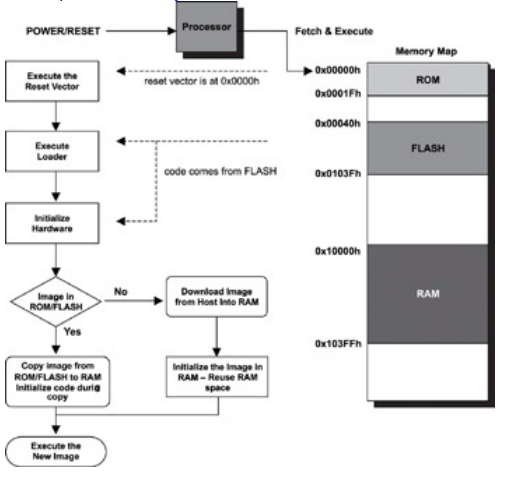
\includegraphics[scale=1]{dados/figuras/InicializacaoBoot.png}
     \caption{Processo de inicialização de um sistema embarcado.\newline Fonte:\cite{Qing2003}}
     \label{fig:INICIALIZAÇÃO}
\end{figure}

Uma imagem executável possui seções de dados inicializados e não inicializados. Essas seções são ambas legíveis e graváveis. Essas seções precisam residir na RAM, assim sendo são copiadas da memória flash para a RAM como parte do sistema de inicialização. A seção de dados inicializados (chamadas pelo \linker de .data e .sdata) contém os valores iniciais para as variáveis globais e estáticas. O contéudo dessa seção, portanto, faz parte da imagem executável final e é transferido completamente pelo \loader. Por outro lado, o contéudo da seção de dados não inicializado (chamado pelo \linker de .bss e .sbss) é vazio. O \linker reserva espaço para essa seção no mapa de memória. As informações de alocação dessas seções, como o tamanho da seção e o endereço de execução da seção, são parte do cabeçario da seção. É trabalho do \loader obter essas informações dos cabeçarios de seção e alocar a mesma quantidade de memória na RAM durante o processo de carregamento. O \loader coloca essas seções na RAM de acordo com o endereço de execução das seções.

Uma imagem executável provavelmente possui constantes. Os dados das contantes são parte da seção chamada pelo \linker de .const, que é somente leitura. Sendo assim, é possível manter a seção .const na memória somente de leitura durante a execução do programa. Constantes de acesso frequente, como tabelas de \textit{lookup}, necessitam ser transferidas para a RAM para melhorar o desempenho do sistema.

O próximo passo no processo de inicialização do sistema é o \loader inicializar os dispositivos do sistema. Apenas os dispositivos necessários são inicializados nesta etapa. Em outras palavras, um dispositivo é inicializado na medida em que um subconjunto necessário dos recursos e recursos do dispositivo estejam ativados e operacionais. Geralmente, os dispositivos são parte da interface de entrada e saida do sistema, portanto, esses dispositivos são completamente iniciados quando existe a necessidade de se fazer \download de uma imagem de outro local.

Agora o \loader esta pronto para transferir a imagem da aplicação para o sistema alvo. A imagem da aplicação pode conter um RTOS, um \textit{kernel}, e os demais códigos das aplicações que o desenvolvedor necessita.


%Conhecer o processo de inicialização dos sistemas embarcados, também chamado de \boot, é muito importante para nos dar noção sobre quando e como entrará em execução tanto a aplicação final, quanto o bootloader.
%Dependendo do fabricante do \textit{chip} o \boot pode ser diferente, porém geralmente ele segue a mesma linha de execução, podendo ou não ter interfaces físicas para mudar a origem do \boot. Algumas placas da ST \cite{ST2019}, contém um mecanismo chamado de \textit{physic remap}, para que o \boot ocorra a partir de outras memórias e não da Flash, que é a padrão \cite{Noviello2018}.

%Como dito por \citeonline{Beningo2015}, o fluxo padrão de \boot do sistema consiste em, após a tensão de referência de um microcontrolador se estabilizar, o processador procura pelo vetor de \textit{reset}, para a obter a localização da instrução de iniciação na Flash. O vetor de reset esta localizado em um endereço especial da memória FLASH, geralmente no início. Como pode ser visto na imagem \ref{MAP_PIC24F16KLXXX} que contém o mapa de memória do MCU (\textit{microcontroller unit}) PIC24F16KLXXX, o vetor de \textit{reset} se encontra no endereço 0x0002.

%\begin{figure}[H]
 %   \scriptsize
 %    \centering
     %\includegraphics[scale=1]{dados/figuras/%ResetVector.jpg}
     %\caption{Mapa de memória do MCU PIC24F16KLXXX.\newline Fonte: \cite{Beningo2015}}
     %\label{MAP_PIC24F16KLXXX}
%\end{figure}

%Então o endereço contido no vetor de \textit{reset} é carregado pelo microcontrolador, e a instrução contida neste endereço é carregada e executada pelo processador. Essa instrução ainda não é a \textit{main} que foi desenvolvida pelo projetista, ela é somente uma instrução de como o MCU irá iniciar. Esta instrução geralmente tem como função copiar o \textit{Vector Table} que esta na memória FLASH para a RAM, copiando e escrevendo em um endereço determinado pelo arquivo de \linker.

%As variáveis que são inicializadas durante o tempo de compilação que estão armazenadas na seção \textit{.data} do arquivo de \linker são então gravadas na memória RAM, e as variáveis não inicializadas explicitamente ou iniciadas com zero que estão na seção \textit{.bss} do arquivo de \linker, são guardadas na memória RAM. O MCU então copia funções que estão na FLASH para a RAM, essa etapa é opcional, o projetista tem que determinar se alguma função deve necessariamente ser executada a partir da memória RAM. 

%Todo esse processo é chamado de \textit{"C Copy Down"}, que faz a preparação do ambiente para iniciar uma aplicação, após essa etapa ser concluída o MCU pode então chamar a função \textit{main}, que é a \firmware principal do sistema desenvolvido pelo projetista. Toda a sequência padrão de \textit{boot} pode ser observada na \autoref{Seq_Boot}.

%\begin{figure}[H]
 %   \scriptsize
  %   \centering
   %  
\includegraphics[scale=1]{dados/figuras/ToDo.jpg}
    % \caption{Sequencia de Boot.}
     %\label{Seq_Boot}
%\end{figure}

%É possível alterar a função da tarefa contida no vetor de \textit{reset} no arquivo de \linker, fazendo com que o MCU passe pelo processo de \textit{C Copy Down}, preparando o sistema para outra função diferente da aplicação principal do sistema embarcado, como é utilizado na criação de um \bootloader para a atualização de \firmware.













\subsection{BOOTLOADER}
O \bootloader é um \textit{software} que, tem como responsabilidade a atualização do \firmware do sistema, operação também conhecida como \textit{in-aplicattion programing} (IAP). Reside em uma área protegida da memória, geralmente colocado no início da flash ou na ROM, e é o primeiro \textit{software} a ser executado após o \textit{reset} ou iniciação do sistema.
É desenvolvido para receber comandos via periféricos de comunicação como: UART, I2C, SPI, CAN e Ethernet, e entender o mapa de memória do microcontrolador \cite{DavesDurlin2013}. A \autoref{Diag_Bootloader} mostra como geralmente fica alocado um \bootloader e o \firmware na memória.
% que são usados para trocar do firmware do MCU e recebimento do novo código de aplicação. Frequentemente é necessário um programa externo para dar esses comandos ao bootloader \cite{Noviello2018}.

\begin{figure}[H]
    \scriptsize
     \centering
     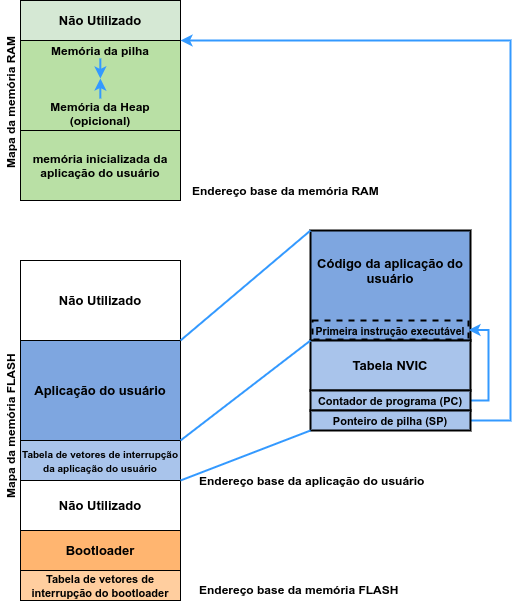
\includegraphics[scale=0.7]{dados/figuras/DiagBootloaderOriginal.png}
     \caption{Alocação do bootloader e firmware nas memórias flash e ram.\newline Fonte:\cite{DavesDurlin2013}}
     \label{Diag_Bootloader}
\end{figure}

Sua função se resume geralmente a: comunicar-se com outro servidor, ler os arquivos enviados pelo \textit{host}, atualizar o \firmware de seu microcontrolador, e iniciar este novo \software. 
Pode conter instruções e comandos definidos pelo projetista para somente o circuito integrado em uso, impossibilitando a utilização do mesmo código em outras placas.
%Sendo desenvolvidos exatamente para o \textit{hardware} que serão empregados,
Portanto, é uma peça de \textit{software} que não é portável para várias plataformas. A \autoref{FluxoBootloader} mostra o funcionamento de um bootloader padrão. 

\begin{figure}[H]
    \scriptsize
     \centering
     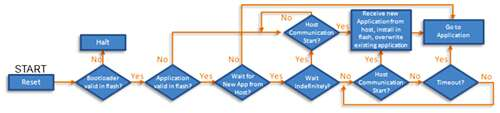
\includegraphics[scale=0.9]{dados/figuras/FluxoBootloader.jpg}
     \caption{Fluxograma de operações de um bootloader.}
     \label{FluxoBootloader}
\end{figure}



Os sistemas microcontrolados STM32 vem de fábrica com um \bootloader pré programado na ROM. Este \bootloader pode utilizar diversos periféricos de comunicação, e para cada periférico diferente a ST padronizou diferentes protocolos que permitem várias operações, como: obter o ID do chip, escrever e ler bytes na RAM e memória flash, apagar setores das memórias, ativar áreas de proteção na memória e pular para o código principal do sistema \cite{Noviello2018}.

É possível ser criado um \bootloader customizado com diversas funções adicionais, uma frequentemente usada é o uso do bootloader para descriptografar firmwares que podem chegar de via \textit{internet}, para se garantir a segurança e origem do \firmware, assim após esse processo o sistema pode substituir o \software anterior pelo recebido. 



\subsection{LINKER}

Segundo \citeonline{Qing2003}, os arquivos de uma aplicação são processados pelo compilador e \textit{assembler}. Criando assim os arquivos objetos, que contém os códigos de máquina binários(\textit{machine binary code}) e dados de programa (\textit{program data}). O \textit{archive utility} concatena uma coleção de arquivos objetos para formar uma biblioteca. Então o \linker obtém esses arquivos objetos como entrada e produz ou um arquivo executável, ou um arquivo objeto que pode ser utilizado em outro \linker com outros arquivos objetos. O arquivo de comandos de \linker (\textit{linker command file}) orienta o \linker em como combinar esses diferentes arquivos objetos e aonde colocar o código binário e os dados no sistema embarcado alvo. Assim podemos concluir que, a função principal de um \linker é combinar múltiplos arquivos objetos em um maior arquivo objeto relocável, um arquivo objeto compartilhado ou uma imagem executável final. Esse processo pode ser observado na \autoref{linker}.

\begin{figure}[H]
    \scriptsize
     \centering
     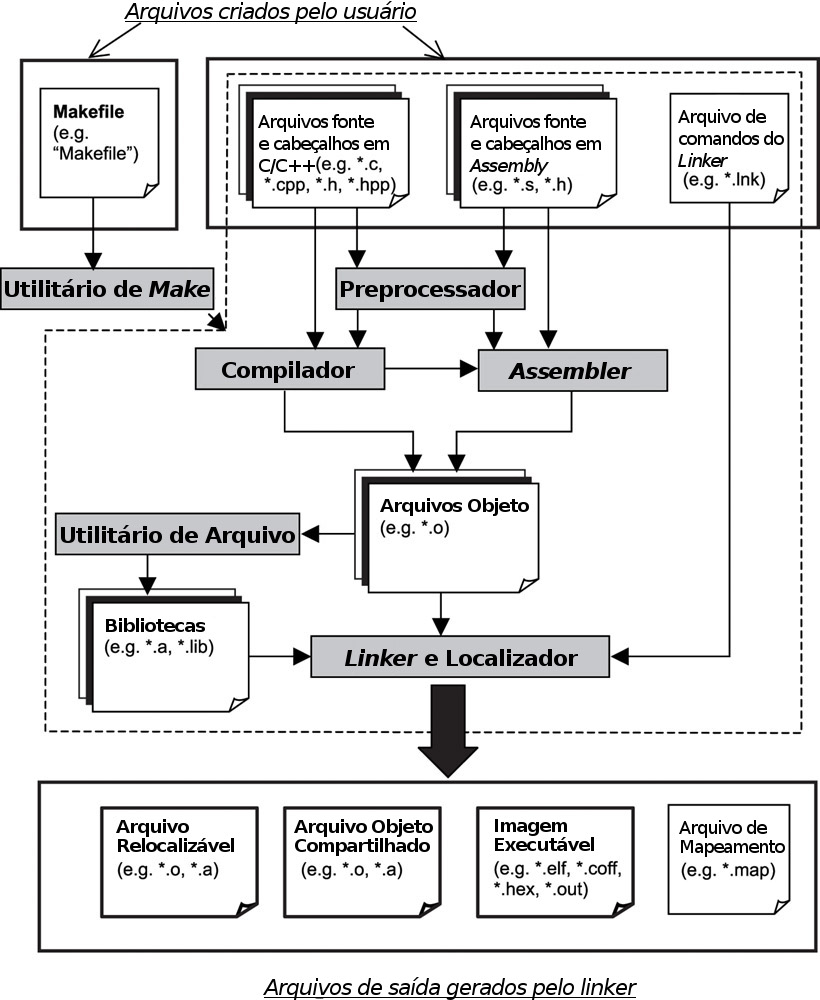
\includegraphics[scale=1]{dados/figuras/Linker.png}
     \caption{Criando um arquivo de imagem para um sistema operacional alvo.\newline Fonte:\cite{Qing2003}}
     \label{linker}
\end{figure}

%Durante a compilação de um arquivo fonte, o compilador cria uma tabela de simbolos contendo os simbolos globais e também as referencias para simbolos externos. O processo de \textit{linking}é feito pelo linker envolvendo a resolução de simbolos e relocação de simbolos.
%melhorar esse paragrafo, pagina 22 Qing

%A resolução de simbolos é o processo em que o linker análisa cada arquivo objeto e determina para cada um, em qual outro arquivo ou arquivos objetos, o simbolo esta definido. Quando um simbolo externo esta definido em uma biblioteca estática, o linker copia o arquivo objeto da biblioteca e o escreve na imagem final.

%A relocação de símbolos é o processo em que o linker mapeia a referência desses símbolos para o local de sua definição. O linker modifica o codigo de máquina do arquivo objeto com o intuito de que o código referenciado pelo simbolo reflita o verdadeiro endereço designado a esse símbolo. A tabela de relocação diz ao linker aonde no código do programa aplica a ação de relocação. Cada entrada na tabela de relocação contem a referência para a tabela de símbolos. Utilizando esta referência, o linker pode recuperar o verdadeiro endereço do símbolo e aplicar em determinada parte do programa, como especificado na tabela de relocação. é possivel que a tabela de relocação contenha tanto o endereço do símbolo, quanto a informação da localização em que ele precisa ser realocado. Neste caso, não existe referencia entre as tabelas de relocação e de símbolo.

%A figura \ref{} mostra esses dois processos de forma simplificada.

%\begin{figure}[H]
%    \scriptsize
%     \centering
%     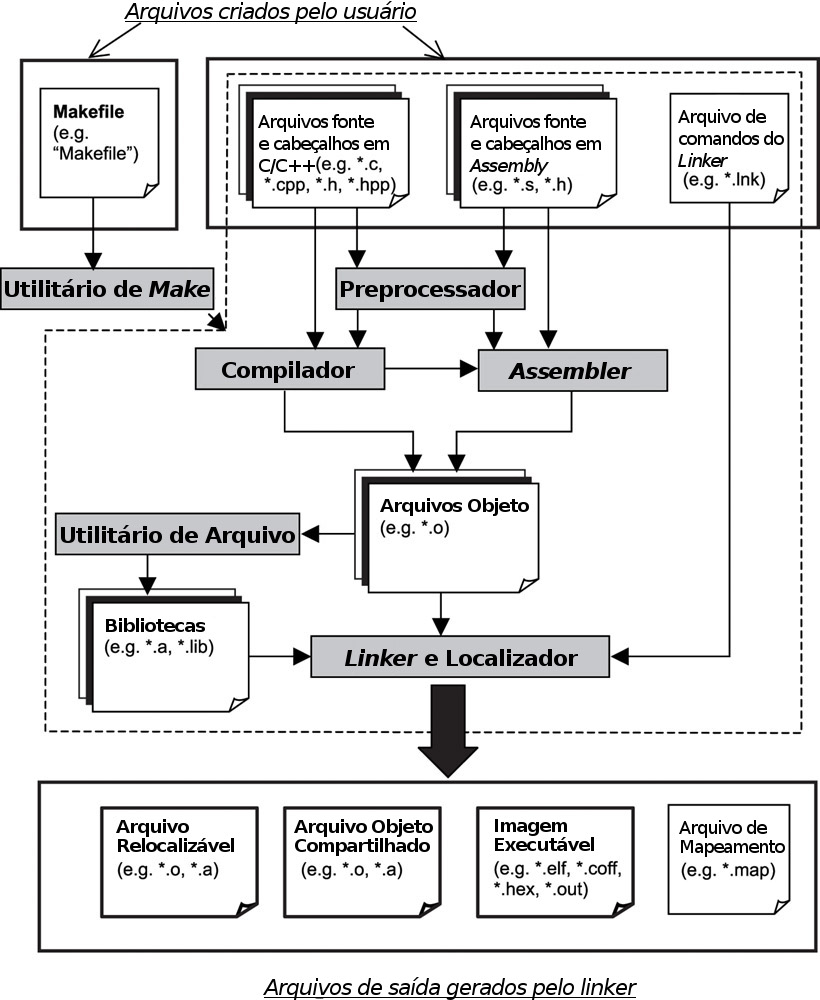
\includegraphics[scale=1]{dados/figuras/Linker.png}
%     \caption{Criando um arquivo de imagem para um sistema operacional alvo.\newline Fonte:\cite{Qing2003}}
%     \label{linker}
%\end{figure}

O \linker precisa combinar esses arquivos objetos e fundir as seções de diferentes arquivos em um segmento de programa. Esse processo cria uma única imagem executável para o sistema embarcado alvo. O desenvolvedor utiliza comandos de \linker (chamados de \textit{linker directives}) para controlar como o \linker combina essas seções e aloca seus segmentos no sistema alvo. As diretivas de \linker ficam contidas no arquivo de comando de \linker. O objetivo de criar esse arquivo de comando de \linker é para que o desenvolvedor de sistemas embarcados possa mapear a imagem executável para o \textit{hardware} alvo de forma precisa e eficiente. 

\begin{figure}[H]
    \scriptsize
     \centering
     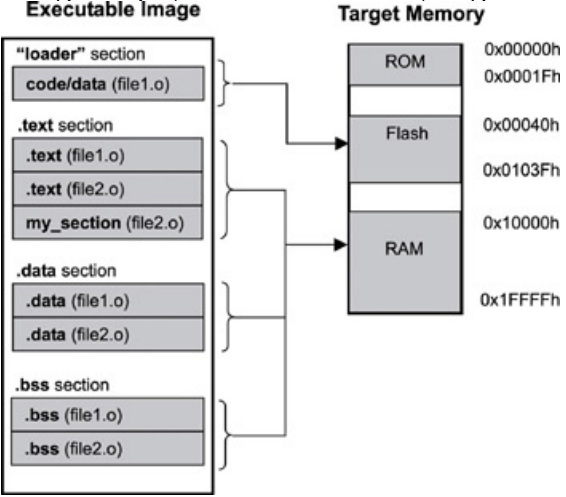
\includegraphics[scale=0.7]{dados/figuras/Linker4.png}
     \caption{Mapeando uma imagem executável em um sistema alvo.\newline Fonte:\cite{Qing2003}}
     \label{linker}
\end{figure}







%\section {COMUNICAÇÃO CLIENTE-SERVIDOR}

%Segundo \citeonline{Kurose2010}, um programa cliente é um programa que funciona em um sistema final, que solicita e recebe um serviço de um programa servidor, que funciona em outro sistema final. Uma vez que o programa cliente é executado em um computador e o programa servidor, é executado em outro, aplicações cliente-servidor são, por definição, aplicações distribuidas. O programa cliente e o servidor interagem enviando mensagens um para o outro pela internet. Neste nivel de abstração, os roteadores, enlaces e outros componentes da internet funcionam como uma caixa-preta que transferem mensagens entre os componentes distribuidos, comunicantes, de uma aplicação.

\section{TCP}

Segundo \citeonline{tanenbaumRedes}, O TCP (\textit{Transmission Control Protocol}) foi projetado especificamente para oferecer um fluxo de bytes fim a fim confiável em uma inter-rede não-confiável. Uma inter-rede é diferente de uma única rede porque suas diversas partes podem ter topologias, larguras de banda, retardos, tamanhos de pacotes e outros parâmetros totalmente diferentes. O TCP foi projetado para se adaptar dinamicamente às propriedades da inter-rede e ser robusto diante de muitos categorias de falhas que podem ocorrer.

Cada máquina compatível com TCP tem uma entidade de transporte TCP, que pode ser um procedimento de biblioteca, um processo do usuário ou parte do núcleo. Em todos os casos, ele gerencia fluxos e interfaces TCP para a camada IP. Uma entidade TCP aceita fluxos de dados de usuários provenientes de processos locais, divide-os em partes de no máximo 64 KB e envia cada parte em um datagrama IP distinto. Quando os datagramas IP que contem dados TCP chegam a uma maquina, eles são enviados à entidade TCP, que restaura o fluxo de bytes originais.

A camada IP não oferece garantia que os datagramas serão entregues de forma apropriada, portanto, cabe ao TCP administrar os timers e retransmiti-los sempre que necessário. Os datagramas também podem chegar fora de ordem, o TCP também terá que os reorganizar em mensagens na sequência correta. Neste trabalho será utilizada a biblioteca LwIP para a implementação da entidade de transporte TCP.

\subsection{LWIP}
%Com a necessidade de se obter os binários dos códigos do novo firmware o sistema irá se utilizar da biblioteca amplamente conhecida e utilizada LWIP.
A Biblioteca LwIP é uma implementação do protocolo TCP/IP, focada em ser pequena e portável, reduzindo a utilização de recursos como memória RAM e ainda tendo um TCP completo, se tornando adequada para sistemas embarcados. Foi originalmente desenvolvida por Adam Dunkels nos laboratórios da \textit{Computer and Networks Architectures} (CNA), no Instituto Sueco de Ciência da Computação (SICS) e agora é desenvolvido e mantido por uma rede mundial de desenvolvedores \cite{LWIP}.

Possui três \textit{Aplication Programing interfaces} (APIs):
\begin{itemize}
\item RAW API (API Crua): É a API nativa do LwIP, possui a melhor desempenho e o menor tamanho de código, porém torna o desenvolvimento de aplicações mais complexo.
\item Netconn API: É uma API sequencial de alto nível que requer um sistema operacional de tempo real (RTOS). Habilita operações com múltiplas \textit{threads}.
\item BSD Sockets API: API de \textit{sockets} de Berkeley, desenvolvida em cima da API Netconn.
\end{itemize}





\subsection{MBED TLS}
A biblioteca mbed TLS foi desenvolvida para se integrar facilmente a aplicações embarcadas existentes, e fornecer os blocos de construção para uma comunicação segura, criptografia e gerenciamento de chaves. Como o seu intuito é ser o mais flexível possível, permite que sejam integrados ao sistema somente as funcionalidades necessárias, diminuindo assim o tamanho total que a biblioteca ocuparia no sistema \cite{mbedtls}.

A \autoref{mbedtlsFig} ilustra como a biblioteca cria uma camada intermediaria entre a aplicação final e a camada TCP/IP.

\begin{figure}[H]
    \scriptsize
     \centering
     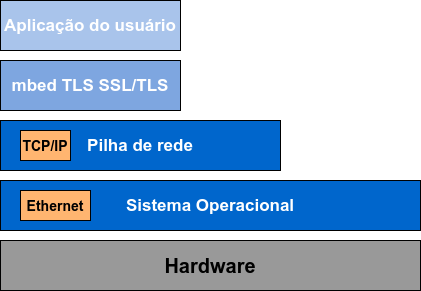
\includegraphics[scale=1]{dados/figuras/mbedtls.png}
     \caption{Pilha de comunicação.\newline Fonte:\cite{mbedtls}}
     \label{mbedtlsFig}
\end{figure}



%\section{CARTÃO SD}
\section{SISTEMA DE ARQUIVO FAT}

Segundo \citeonline{tanenbaumSO}, o sistema de arquivo FAT (\textit{File Allocation Table}) é implementado por meio de uma alocação de memória encadeada usando uma tabela na memória. Nesta organização, o bloco de memória inteiro esta disponível para dados. Além disso, o acesso aleatório é muito mais fácil. Mesmo que o encadeamento ainda tenha que ser seguido para encontrar determino deslocamento dentro do arquivo, ele esta inteiramente na memória. De modo que, pode ser seguido sem necessidade nenhuma de referenciar o disco.

A \autoref{FAT} ilustra como é a tabela, mostrando que o arquivo A inicia-se no bloco 4 e segue o encadeamento até o seu fim, assim como o arquivo B que se inicia no bloco 6. Ambos terminam com um marcador especial que no caso é o número -1.

\begin{figure}[H]
    \scriptsize
     \centering
     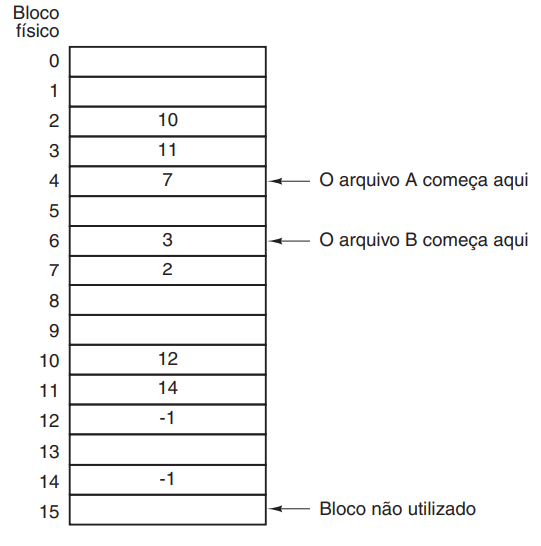
\includegraphics[scale=0.7]{dados/figuras/FAT.png}
     \caption{Alocação encadeada usando tabela de alocação de arquivo.\newline  Fonte:\cite{tanenbaumSO}}
     \label{FAT}
\end{figure}

A principal desvantagem deste método é que a tabela inteira precisa estar na memória o tempo todo. Com um disco de 20 GB e um tamanho de bloco de 1 KB, a tabela precisa de 20 milhões de entradas, uma para cada um dos 20 milhões de blocos do disco. Cada entrada tem de ter no mínimo 3 bytes para manter o endereço dos blocos. Para facilitar sua pesquisa, as entradas acabam ocupando 4 bytes. Assim, a tabela ocupará 60 MB ou 80 MB de memória principal o tempo todo, dependendo do sistema para ser otimizado para espaço ou para tempo.

\subsection{FATFS}

FatFs é um modulo genérico de um sistema de arquivo FAT/exFAT, para pequenos sistemas embarcados. É escrito em conformidade com a ANSI C (C89) e é completamente separado da camada de entrada e saída do sistema, portanto é independente da plataforma utilizada. A \autoref{FatFS}


\begin{figure}[H]
    \scriptsize
     \centering
     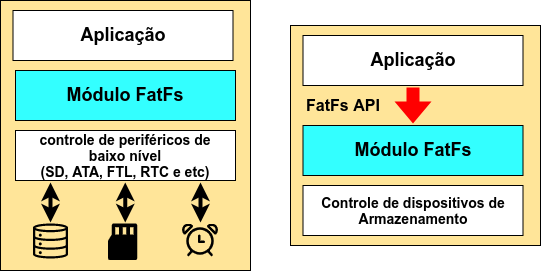
\includegraphics[scale=0.5]{dados/figuras/fatfs.png}
     \caption{Posição da biblioteca FatFs na aplicação.\newline  Fonte:\cite{FATFS}}
     \label{FatFS}
\end{figure}

%\section{SERVIDORES HTTP}

%É uma boa prática iniciar cada novo capítulo com um breve texto introdutório (tipicamente, dois ou três parágrafos) que deve deixar claro o quê será discutido no capítulo, bem como a organização do capítulo.
%Também servirá ao propósito de "amarrar"{} o conteúdo deste capítulo com o conteúdo do capítulo imediatamente anterior.


\section{TRABALHOS CORRELATOS}

Foram identificados três trabalhos correlatos.

%pode ter latencia de interrupção porem deve ser controlada

\begin{itemize}

    \item \textbf{Firmware over the air for automotive, Fotamotive}: Esse trabalho introduz uma solução para atualização de veículos com a ajuda de fabricantes de equipamentos originais para reduzir custos, \textit{recalls} aumentar a qualidade, facilitar as atualizações e controlar melhor a frota de veículos no mercado. Essa solução consiste em atualizar a unidade de controle do motor por meio de métodos OTA, sem a necessidade de uma conexão física com o veículo \cite{Odat2014}.

    \item \textbf{Firmware over the air for home cybersecurity in the Internet of Things}: Esse trabalho descreve a utilização de um método de atualização de \firmware para roteadores caseiros, utilizando sistemas de gerenciamento de rede e de suporte de operações de fornecedores de acesso à \textit{internet} \cite{Teng2017}.
    
    \item \textbf{Internet of Things: Over-the-Air (OTA) firmware update in Lightweight mesh network protocol for smart urban development}: Esse trabalho introduz um novo sistema de atualização de \firmware \textit{Over-The-Air} (OTA) baseado no protocolo de rede \textit{Lightweight mesh}, que prove descoberta de rotas, estabelecimento e um protocolo de malha de baixa potência \cite{Chandra2016}.

\end{itemize}

Como observado, todos os trabalhos correlatos tem um objetivo único e diferente para a aplicação de sua atualização OTA, enquanto este trabalho tem como meta produzir um sistema que pode abranger diferentes aplicações.